% Created 2016-11-04 Fri 12:52
\documentclass[presentation]{beamer}
\usepackage[utf8]{inputenc}
\usepackage[T1]{fontenc}
\usepackage{fixltx2e}
\usepackage{graphicx}
\usepackage{longtable}
\usepackage{float}
\usepackage{wrapfig}
\usepackage{rotating}
\usepackage[normalem]{ulem}
\usepackage{amsmath}
\usepackage{textcomp}
\usepackage{marvosym}
\usepackage{wasysym}
\usepackage{amssymb}
\usepackage{hyperref}
\tolerance=1000
\institute{Wydział Matematyki i Informatyki UWr}\subtitle{Praca magisterska pod opieką dra hab. Dariusza Biernackiego}
\usetheme{Madrid}
\usecolortheme{}
\usefonttheme{}
\useinnertheme{}
\useoutertheme{}
\author{Łukasz Czapliński}
\date{\today}
\title{Zastosowanie funkcyjnego paradygmatu do tworzenia graficznego środowiska programistycznego}
\hypersetup{
  pdfkeywords={},
  pdfsubject={},
  pdfcreator={Emacs 25.1.1 (Org mode 8.2.10)}}
\begin{document}

\maketitle
\begin{frame}{Outline}
\tableofcontents
\end{frame}

\section{Omówienie problemu}
\label{sec-1}
\begin{frame}[label=sec-1-1]{Ekrany dotykowe jako główna metoda interakcji z komputerem}
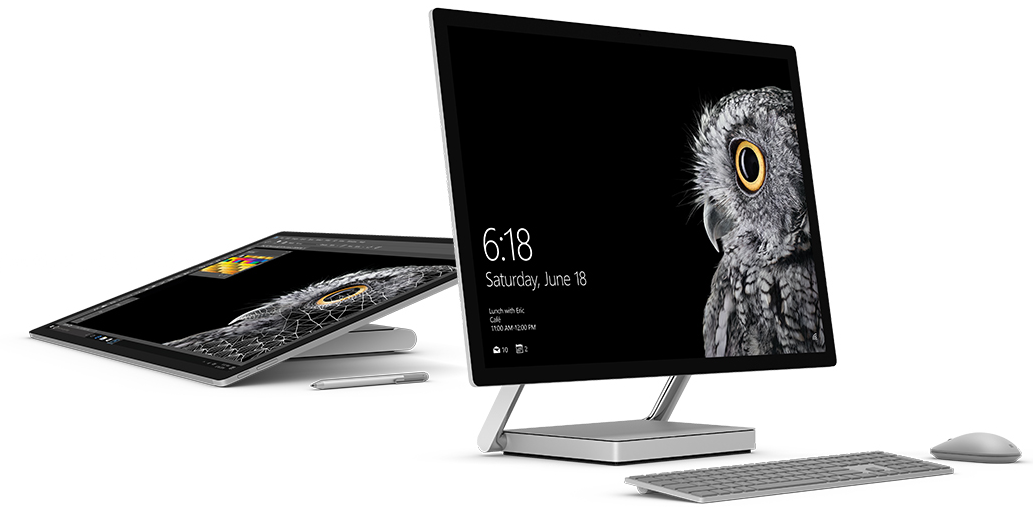
\includegraphics[width=.9\linewidth]{./img/studio.png}
\end{frame}
\begin{frame}[label=sec-1-2]{Rozwiązanie: programowanie przez diagramy}
\begin{figure}[htb]
\centering
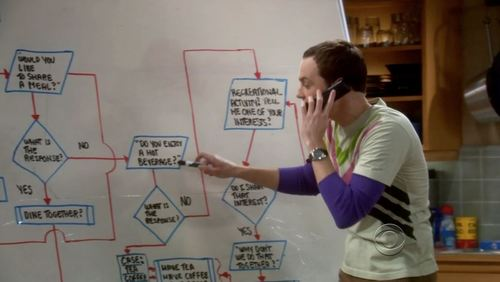
\includegraphics[width=.9\linewidth]{./img/whiteboard.jpg}
\caption{\small{Copyright Warner Bros. Television}}
\end{figure}
\end{frame}
\begin{frame}[label=sec-1-3]{Graficzne języki programowania - Scratch}
\begin{columns}
\begin{column}{0.4\textwidth}
\begin{itemize}
\item Lifelong Kindergarten Group, MIT, 2005
\item edukacyjny, dla dzieci w wieku 8-16 lat
\item pozwala na tworzenie interaktywnych scen
\item przypomina układanie puzzli
\end{itemize}
\end{column}
\begin{column}{0.6\textwidth}
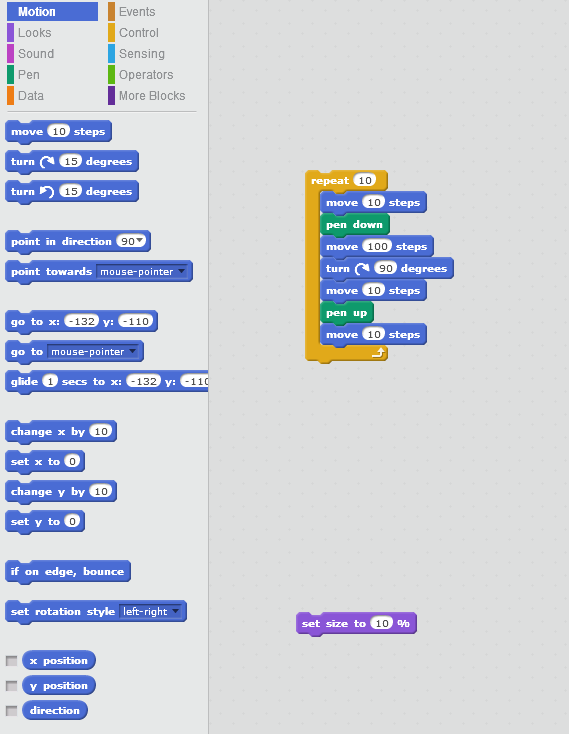
\includegraphics[width=0.8\textwidth]{./img/s-puzzle.png}
\end{column}
\end{columns}
\end{frame}
\begin{frame}[label=sec-1-4]{Graficzne języki programowania - Blueprints}
\begin{columns}
\begin{column}{0.4\textwidth}
\begin{itemize}
\item Unreal Engine, Epic, 2014
\item pisanie poziomów gier
\item dla developerów, nie programistów
\item łączenie węzłów - druty symbolizują przepływ danych oraz wykonanie programu
\end{itemize}
\end{column}
\begin{column}{0.6\textwidth}
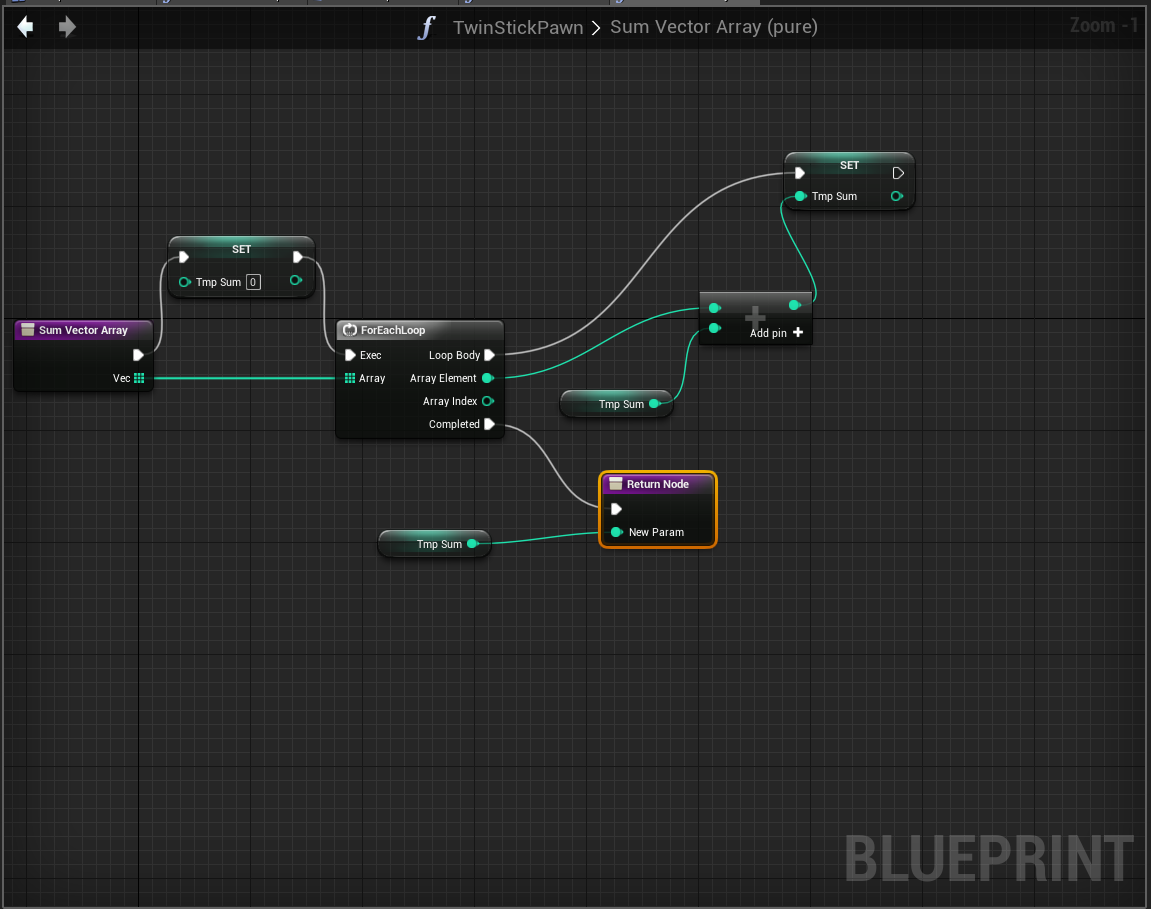
\includegraphics[width=.9\linewidth]{./img/b-wires.png}
\end{column}
\end{columns}
\end{frame}
\begin{frame}[label=sec-1-5]{Graficzne języki programowania}
\begin{block}{Zalety}
\begin{itemize}
\item Prostsze w nauce
\item Doskonałe dla ekranów dotykowych
\item Dopasowane do swoich nisz
\end{itemize}
\end{block}
\begin{block}{Wady}
\begin{itemize}
\item Brak graficznego języka programowania ogólnego zastosowania
\item Egzotyczne sposoby zapisu
\end{itemize}
\end{block}
\end{frame}
\begin{frame}[label=sec-1-6]{Przeszkody w zdobyciu popularności - Edytory}
\begin{columns}
\begin{column}{0.4\textwidth}
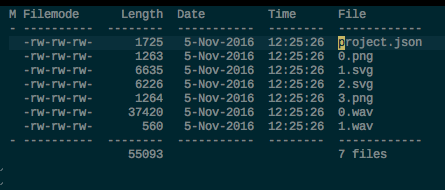
\includegraphics[width=.9\linewidth]{./img/scratch-project-listing.png}
\end{column}
\begin{column}{0.6\textwidth}
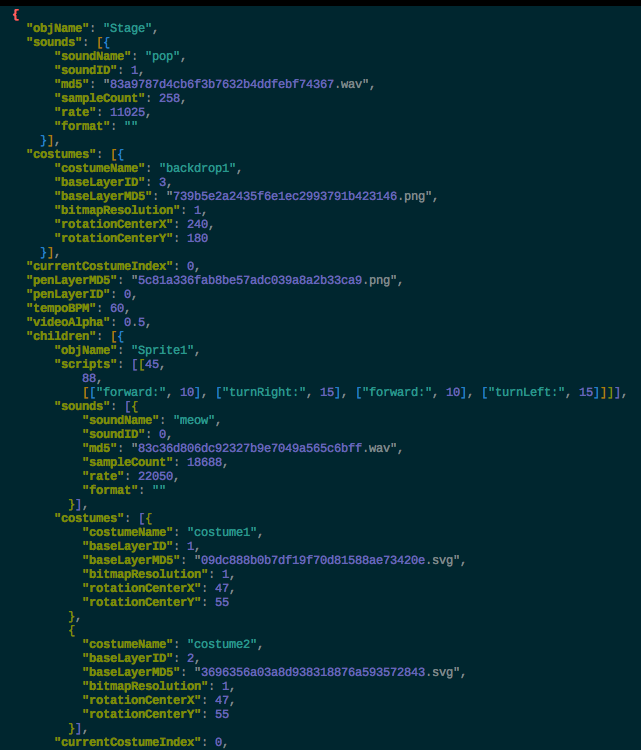
\includegraphics[width=.9\linewidth]{./img/scratch-project-json.png}
\end{column}
\end{columns}
\end{frame}
\begin{frame}[label=sec-1-7]{Przeszkody w zdobyciu popularności - Systemy kontroli wersji}
\begin{block}{Pliki projektu są wykrywane jako binarne.}
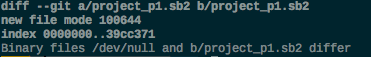
\includegraphics[width=.9\linewidth]{./img/scratch-git-reaction.png}
\end{block}
\end{frame}
\begin{frame}[label=sec-1-8]{Przeszkody w zdobyciu popularności - Code Review}
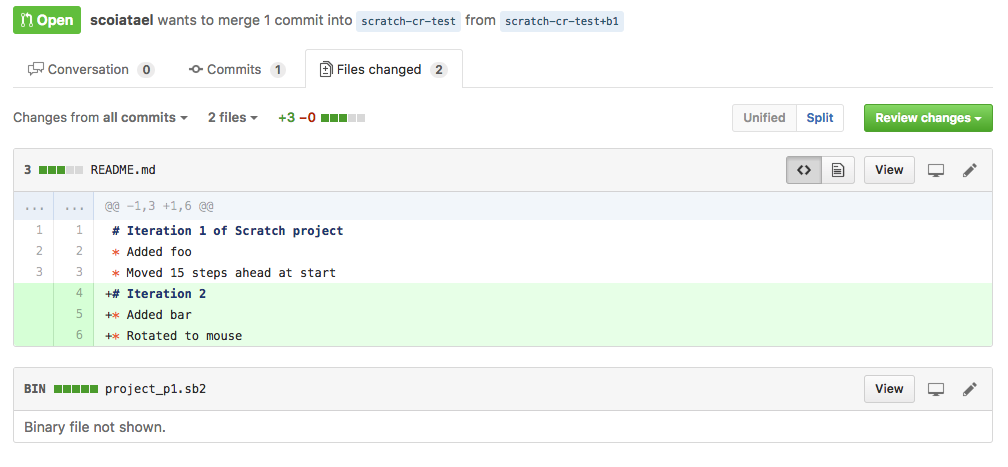
\includegraphics[width=.9\linewidth]{./img/scratch-cr.png}
\end{frame}
\section{Cel}
\label{sec-2}
\begin{frame}[label=sec-2-1]{Cel}
\begin{itemize}
\item Graficzne środowisko programistyczne
\item Łatwa integracja z isniejącym systemem - znany język
\item Łatwa integracja z isniejącym systemem - czytelny format zapisu
\item Przygotowane do programowania na ekranach dotykowych
\item Integracja z narzędziami dla programistów
\end{itemize}
\end{frame}
\section{Realizacja}
\label{sec-3}
\begin{frame}[label=sec-3-1]{Realizacja: Język - Clojure}
\end{frame}
\begin{frame}[label=sec-3-2]{Realizacja: Technologia - Electron + Clojurescript}
\end{frame}
\begin{frame}[label=sec-3-3]{Realizacja: Integracja z REPLem}
\end{frame}
\section{Wyniki}
\label{sec-4}
\begin{frame}[label=sec-4-1]{Wyniki - Jarvis}
\end{frame}
\section{Wnioski i wyzwania na przyszłość}
\label{sec-5}
\begin{frame}[label=sec-5-1]{Problemy}
\begin{itemize}
\item Brak wsparcia dla wszystkich struktur Clojure
\item Brak wsparcia dla makr
\end{itemize}
\end{frame}
\begin{frame}[label=sec-5-2]{Możliwe ulepszenia}
\begin{itemize}
\item Inne reprezentacja kodu
\item Lepsza interakcja z użytkownikiem
\end{itemize}
\end{frame}
% Emacs 25.1.1 (Org mode 8.2.10)
\end{document}